\documentclass[12pt]{llncs}



% This is LLNCS.DEM the demonstration file of
% the LaTeX macro package from Springer-Verlag
% for Lecture Notes in Computer Science,
% version 2.4 for LaTeX2e as of 16. April 2010
%
%

% ADDED CUSTOM PACKAGES
% Fonts
\usepackage{mathptmx}
% Layout
\usepackage[margin=20mm]{geometry}
\usepackage{setspace}
\doublespacing
\usepackage{multicol}
\usepackage{bbm}
\usepackage{url}
\bibliographystyle{splncs03}


\usepackage{amssymb,array}
\usepackage{enumitem}


% Maths
\usepackage{amsmath}
\newcommand*\diff{\mathop{}\!\mathrm{d}}
\newcommand*\Diff[1]{\mathop{}\!\mathrm{d^#1}}
\usepackage{algorithm}
\usepackage{algpseudocode}


% Graphics
\usepackage{placeins}
\usepackage{graphicx}
% \graphicspath{{../../Papers/ECML/Images/}}
\usepackage{caption}
\captionsetup{compatibility=false}
\usepackage{subcaption}
\usepackage{tikz} % Essential for Neural Network diagrams



\tikzstyle{state}=[shape=circle,draw=blue!50,fill=blue!20]
\tikzstyle{observation}=[shape=rectangle,draw=orange!50,fill=orange!20]
\tikzstyle{lightedge}=[<-,dotted]
\tikzstyle{mainstate}=[state,thick]
\tikzstyle{mainedge}=[<-,thick]


\usepackage[colorlinks=true,linkcolor=blue,urlcolor=black, bookmarksdepth=2]{hyperref}
\usepackage{bookmark}
\usepackage{comment}
% Custom environments

\newenvironment{Figure}
  {\par\medskip\noindent\minipage{\linewidth}}
  {\endminipage\par\medskip}

%\usepackage{natbib}   
%\newcommand{\citep}{\cite} % remove me when the natbib issue is resolved
%\newcommand{\citet}{\cite} % remove me when the natbib issue is resolved
%\newcommand{\citeyear}[1]{YEAR } % remove me when the natbib issue is resolved

% END CUSTOM PACKAGES

\usepackage{makeidx}  % allows for indexgeneration
\usepackage[draft]{todonotes}
\setlength{\marginparwidth}{1.5cm} % Not a lot of space for notes in margin
% dav's notes
\newcommand{\dzN}[1]{\todo[inline, size=\small, color=yellow!30]{[dz] #1}}
\newcommand{\dzn}[1]{\todo[color=yellow!30]{[dz] #1}}
% ivan's notes
\newcommand{\ikN}[1]{\todo[inline, size=\small, color=orange!30]{[ik] #1}}
\newcommand{\ikn}[1]{\todo[size = \small, color=orange!30]{[ik] #1}}
% steve's notes
\newcommand{\srN}[1]{\todo[inline, size=\small, color=cyan!30]{[sr] #1}}
\newcommand{\srn}[1]{\todo[color=cyan!30]{[sr] #1}}
% ber's notes
\newcommand{\bpN}[1]{\todo[inline, size=\small, color=purple!30]{[bp] #1}}
\newcommand{\bpn}[1]{\todo[color=purple!30]{[bp] #1}}
% theo's notes
\newcommand{\twN}[1]{\todo[inline, size=\small, color=green!30]{[tw] #1}}
\newcommand{\twn}[1]{\todo[color=green!30]{[tw] #1}}
% yunpeng's notes
\newcommand{\ylN}[1]{\todo[inline, size=\small, color=blue!30]{[yl] #1}}
\newcommand{\yln}[1]{\todo[color=blue!30]{[yl] #1}}

% ms's notes
\newcommand{\msN}[1]{\todo[inline, size=\small, color=gray!30]{[ms] #1}}
\newcommand{\msn}[1]{\todo[color=gray!30]{[ms] #1}}

\begin{document}
%
%\setcounter{tocdepth}{4}
%\tableofcontents


%
\pagestyle{headings}  % switches on printing of running heads

%
\mainmatter              % start of the contributions


\title{Signal Detection}
%

%\titlerunning{Hamiltonian Mechanics}  % abbreviated title (for running head)
%                                     also used for the TOC unless
%                                     \toctitle is used
%
\author{Ivan Kiskin\inst{1,2}}
%
% \authorrunning{Ivar Ekeland et al.} % abbreviated author list (for running head)
%
%%%% list of authors for the TOC (use if author list has to be modified)
% \tocauthor{Ivar Ekeland, Roger Temam, Jeffrey Dean, David Grove,
% Craig Chambers, Kim B. Bruce, and Elisa Bertino}
%
\institute{University of Oxford, Department of Engineering, Oxford OX1 3PJ, UK, \\
\and
\email{\textrm{ikiskin@robots.ox.ac.uk}}, 
}
% \and
% \email{\textrm{\{}ikiskin, ber, dzilli, sjrob\textrm{\}}@robots.ox.ac.uk}, 
% % \and
% % \email{ber@robots.ox.ac.uk}\\
% \institute{test, \\
% \and
% \email{theo.windebank@stcatz.ox.ac.uk}}\\
% \and
% \email{dzilli@robots.ox.ac.uk}\\
% \and
% \email{marianne.sinka@zoo.ox.ac.uk}
% % \and
% \email{sjrob@robots.ox.ac.uk}
%\and
%\institute{University of Oxford, Department of Zoology, Oxford OX2 6GG, UK}}


\maketitle              % typeset the title of the contribution




\section{Introduction}

Signal detection is a very broad research area with contributions from a wide range of academic disciplines. We define signal detection theory as \emph{``a means to quantify the ability to discern between information-bearing patterns and random patterns that distract from the information (called noise, consisting of background stimuli and random activity of the detection machine)"}\ikn{Write own def/find good source}. The aim of the DPhil is to progress the state-of-art by working on specific real-world applications.  The motivation to excel in the application aligns with the need to innovate algorithms or architectures.

This literature review critically covers contributions to signal processing and deep learning in the context of signal detection.
The research is thus  examined in chronological order, examining the progression of the state of the art in specific fields. We narrow down our focus to audio signals and highlight the potential areas in need of further improvements, forming the basis of our research efforts. Section \ref{sec:speechrecognition} focuses specifically on the speech recognition field, due to its competitive nature and associated rich publication record as well as the closeness to our chosen application domains. The progress in speech recognition state of art was fuelled by both industry and academia due to its importance in human-machine interaction systems, that arguably are essential to general artificial intelligence [cit].

Section \ref{sec:imagerecognition} focuses on image recognition, the most competitive field and resultant driver in the scientific literature.
Our focus then shifts to birdsong recognition and acoustic event detection in Sections \ref{sec:birdrecognition} and \ref{sec:AED} as fields where innovation was driven by progress in both speech and image recognition.

We further highlight detection methods from traditional signal  processing literature  that show most potential promise of transferability to our application in Section  \ref{sec:traditional}.

Finally, we outline how reviewed methodology directly applies to our application of mosquito detection, which falls within the scope of noisy audio signal detection.


The literature review is followed by the research proposal which includes a concise summary of completed work, future work, and a risk assessment. Future work is broken down into short, medium and long-term goals in Section \ref{sec:proposal}. We conclude with .... in Section \ref{sec:conclusion}.



\section{Speech Recognition}
\label{sec:speechrecognition}
Due to its significance in academia and industry [cite], much attention is given to the field of speech recognition. Speech recognition has been a prominently researched field due to its critical role in human-machine interactions. The ability to accurately transcribe spoken text would influence a diverse range of applications, and hence has been the subject of prominent study. 

We choose to concentrate on work since the 1990s, as it forms the basis of modern methods which are more applicable to our/current research. Major breakthroughs in early methods came from a paradigm shift to more statistics-based methods, such as the Hidden Markov Model (HMM) \cite{juang2005automatic}. An HMM is a statistical model, where the system is modelled as a Markov process with discrete latent variables. An HMM can be interpreted as an extension of a mixture model in which latent variables are related by a Markov process \cite{bishop2006pattern}. The discrete multinomial latent variables describe which component of the mixture is responsible for generating the corresponding observation.

By defining a state transition matrix (between states $s_i$) and the state output distribution, the HMM can be used as a generative classifier (for predicting $y_i$). An example scenario is given in Figure \ref{fig:HMM}.

\begin{figure}[htbp]
\begin{center}
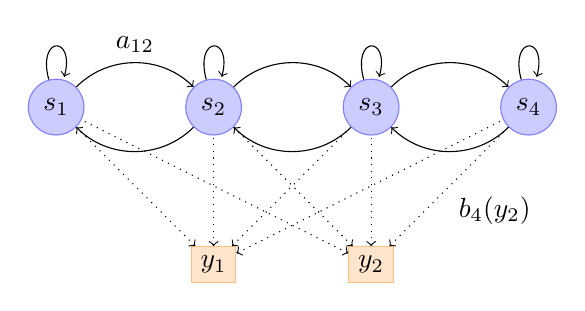
\begin{tikzpicture}[]
% states
\node[state] (s1) at (0,2) {$s_1$}
    edge [loop above]  ();
\node[state] (s2) at (2,2) {$s_2$}
    edge [<-,bend right=45] node[auto,swap] {$a_{12}$} (s1)
    edge [->,bend left=45] (s1)
    edge [loop above] ();
\node[state] (s3) at (4,2) {$s_3$}
    edge [<-,bend right=45] (s2)
    edge [->,bend left=45] (s2)
    edge [loop above] ();
\node[state] (s4) at (6,2) {$s_4$}
    edge [<-,bend right=45] (s3)
    edge [->,bend left=45] (s3)
    edge [loop above] ();
% observations
\node[observation] (y1) at (2,0) {$y_1$}
    edge [lightedge] (s1)
    edge [lightedge] (s2)
    edge [lightedge] (s3)
    edge [lightedge] (s4);
\node[observation] (y2) at (4,0) {$y_2$}
    edge [lightedge] (s1)
    edge [lightedge] (s2)
    edge [lightedge] (s3)
    edge [lightedge] node[auto,swap] {$b_4(y_2)$} (s4);
\end{tikzpicture}
\end{center}
\caption{An HMM with 4 states which can emit 2 discrete symbols $y_1$ or $y_2$.
$a_{ij}$ is the probability to transition from state $s_i$ to state $s_j$.
$b_j(y_k)$ is the probability to emit symbol $y_k$ in state $s_j$.
In this particular HMM, states can only reach themselves or the adjacent state.}
\label{fig:HMM}
\end{figure}







Prominent contributions \cite{rabiner1993fundamentals} (book, fundamentals of theory etc), [cite2]. The improvements came from the introduction of ... (better theoretical understanding?/more powerful hardware? more data?)
Relevance to general signal detection? However in the absence of phenomes/not wishing to encode a rich library of prior information (linguistics understanding) / perhaps machines do this better than us: Deep learning


\subsubsection{Move towards hybrid DNN-HMM}


Effect of introduction of DL on literature \cite{deng2014achievements}:
Output representation learning:
Designing effective linguistic representations for the output layers of deep networks for ASR. Context-dependent states 1000-30000. Design follows traditional GMM-HMM systems. CD-DNN gave much higher accuracy when large training data supported model capacity. Future: making use of linguistically-guided structured design based on symbolic/phonological units of speech?

Moving towards raw features:
do away with hand-crafted feature engineering. MFCCs led to significant accuracy improvements in GMM/HMM systems despite known loss of information introduced.

\emph{MFCCs, GMMs, and HMMs co-evolved as a way of doing
speech recognition when computers were too slow to explore
more computationally intensive approaches. MFCCs throw
away a lot of the information in the sound wave, but preserve
most of the information required for discrimination. By including
temporal differences, MFCCs partially overcome the
very strong conditional independence assumption of HMMs,
namely that successive frames are independent given the
hidden state of the HMM. The temporal differences also allow
diagonal covariance Gaussians to model the strong temporal
covariances by reducing these particular pairwise covariances
to individual coefficients. As we shall see, a Fourier transform
based filterbank, densely distributed on a mel-scale, is a potential
alternative to MFCCs for models that can easily model
correlated features [7]. \cite{mohamed2012acoustic}}



 Cos transform approx de-correlates feature components, important for use of GMMs with diagonal cov matricies. Does not apply to deep learning models, where strength of deep learning methods in modelling data correlation makes transform reduntant.


``For example, Mohamed et al. (2012a) \cite[firstExampleMovingGMMsectionofHMM/GMMtoDNN]{mohamed2012acoustic} and Li et al., (2012) showed
significantly lowered ASR errors using large-scale DNNs when moving from the MFCC features back to
more primitive (Mel-scaled) filter-bank features. These results indicate that DNNs can learn a better
transformation than the original fixed cosine transform from the Mel-scaled filter-bank features."
Perhaps a move to raw input data (waveform): see end of paragraph

Better optimisation, architectures, transfer learning and noise robustness

\subsubsection{Move towards DNN}

Recently, Deep Neural Networks (DNNs) have achieved tremendous
success in acoustic modeling for large vocabulary continuous
speech recognition (LVCSR) tasks, showing significant gains over
state-of-the-art Gaussian Mixture Model/Hidden Markov Model
(GMM/HMM) systems on a wide variety of small and large vocabulary
tasks 


\cite{dahl2012context}
\emph{We illustrate the key components of our model, describe the procedure for applying CD-DNN-HMMs to LVSR, and analyze the effects of various modeling choices on performance. Experiments on a challenging
business search dataset demonstrate that CD-DNN-HMMs
can significantly outperform the conventional context-dependent
Gaussian mixture model (GMM)-HMMs, with an absolute sentence
accuracy improvement of 5.8 \% and 9.2 \% (or relative error
reduction of 16.0 \% and 23.2 \%) over the CD-GMM-HMMs trained
using the minimum phone error rate (MPE) and maximum-likelihood
(ML) criteria, respectively.}


Historically, the use of rectified linear units to train large networks in computer vision carried over to training DNNs in speech detection, resulting in performance gains relative to DNNs trained with sigmoid units, with further improvement on GMM/HMM systems. \cite{dahl2013improving}




\subsubsection{Final move from DNN to CNN/LSTM}


\subsubsection*{Deep Convolutional Neural Networks for Large-scale Speech Tasks \cite{sainath2015deep}}
\begin{itemize}
	\item Paper focuses on details of implementation -- number of layers, dropout/pooling, choice of activation functions (quite descriptive). 
	\item CNNs on the other hand capture translational invariance with far fewer parameters by averaging the outputs of hidden units in different local time and frequency regions.
	\item Full weight sharing: allowing multiple convolutional layers, encouraging deeper networks (c.f. limited weight sharing: limited to one convolutional layer)
	\item Performance decreasing after more than 2 conv layers
	\item Pooling in time with overlap can thought of as a way to smooth out the signal in time, another form of regularization.
\end{itemize}

\subsubsection{Include LSTM paper}

\subsubsection{Relevance to our application?}\ikn{Not sure if necessary}\srN{put in and make decision later - probably best in}






\section{Bird recognition}
\label{sec:birdrecognition}
BirdCLEF case study. Flesh out main points made in paper lit review. Move from traditional classifiers to Deep Learning

A prominent example of this shift in methodology is the BirdCLEF bird recognition challenge. The challenge consists of the classification of bird songs and calls into up to 1500 bird species from tens of thousands of crowd-sourced recordings. The introduction of deep learning has brought drastic improvements in mean average precision (MAP) scores. The best MAP score of 2014 was 0.45 \cite{goeau2015lifeclef}

1st
MNB TSA, Germany, 4 runs [13]: This participant combined two main
categories of features for the classification: parametric acoustic features (see
openSMILE Audio Statistics) and probabilities of species-specific spectrogram
segments (see Segment-Probabilities)

2nd
The final
classification was then completed thanks to a support vector machine trained on
top of the resulting matching-based representations.




, which was improved to 0.69 the following year when deep learning was introduced, outperforming the closest scoring hand-crafted method that scored 0.58 \cite{joly2016lifeclef}. 


1st: 5-layer CNN CUBE Switzerland


2nd:

MNB from last year but with more experience: still losered







The impressive performance gain came from the utilisation of well-established convolutional neural network practice from image recognition. By transforming the signals into STFT spectrogram format, the input is represented by 2D matrices, which are used as training data. 



\subsubsection*{BirdCLEF 2016 winner: Audio Based Bird Species Identification using
Deep Learning Techniques \cite{sprengel2016audio}}
\begin{itemize}
	\item Convnets on spectrogram chunks, with denoising step
	\item Five conv layers, one dense layer. Every conv layer uses a rectify activation function, followed by a max-pooling layer
	layer. 
	\item No performance benefit from using 1D convolution with height equal to spectral width (frequency)
	\item Used smaller 2D patches instead
	\item Each chunk around 3 seconds in length, acting as a unique training sample for the NN
\end{itemize}

\section{Image recognition}
\label{sec:imagerecognition}
Strong parallels with deep learning methods on sound (spectrogram representation simply an image). More active research area. State-of-art potentially ahead than sound detection [evidence].
\srN{point out that only very recently have techniques from image analysis come into the signal world}


\subsection{Deep Kernel Learning}

From Wilson et. al \cite{wilson2016deep}
\emph{In the experiments, we show that jointly learning all deep kernel parameters has advantages over training a GP applied to the output layer of a trained deep neural network.}

\begin{itemize}
	\item DKL does as well/slightly better than pure CNN for learning MNIST dataset. The CNN significantly outperforms GP, DBN + GP and CNN + GP. Definitely worth investigating using for my own task
\end{itemize}


\section{Acoustic Event Detection}
\label{sec:AED}
(Use this to introduce AED as relevant to our research)

From \cite{espi2015exploiting}:
\emph{Acoustic event detection (AED) is the field that deals
with detecting and classifying these non-speech acoustic
signals, and the goal is to convert a continuous acoustic
signal into a sequence of event labels with associated
start and end times. The field has attracted increasing
attention in recent years including dedicated challenges
such as CLEAR \cite{mostefa2007chil}, and recently D-CASE \cite{giannoulis2013detection}, with tasks
involving the detection of a known set of acoustic events
happening in a smart room or office setting. In addition,
AED applications range from rich transcription in
speech communication \cite{mostefa2007chil,giannoulis2013detection} and scene understanding}



We further examine the progression of the state-of-art in acoustic event detection. An example can be found at the Music Information Retrieval Evaluation eXchange (MIREX). Example tasks include recognising musical chords. This requires detecting a specific composition of frequencies localised in time. Classifying musical instruments that play the same fundamental notes requires detection of the harmonic structure of those notes. 
A study of MIREX concluded that the state-of-art stagnated in variety of such classification and detection tasks (Humphrey et al. \cite{humphrey2013feature}) between 2007 and 2012. 
This was attributed to the use of traditional methods for feature extraction and classification. It was suggested deep learning can help overcome three deficiencies associated with traditional methods: hand-crafted feature design is not sustainable, shallow processing architectures struggle with latent complexity of real-world phenomena, short-time analysis cannot naturally capture higher-level information.
% For example, recognising musical chords requires detecting a specific composition of frequencies localised in time. Classifying musical instruments that play the same fundamental notes requires detection of the harmonic structure of those notes. Based on a study of the MIREX (Music Information Retrieval Evaluation eXchange) it was concluded that the state of art in music informatics has seen decelerating progress in a wide range of classification and detection tasks (Humphrey et al. \cite{humphrey2013feature}) between 2007 and 2012. This was attributed to the use of traditional methods for feature extraction and classification. It was suggested deep learning can help overcome three deficiencies associated with traditional methods: hand-crafted feature design is not sustainable, shallow processing architectures struggle with latent complexity of real-world phenomena, short-time analysis cannot naturally capture higher level information. 
Indeed since the assessment, there has been a paradigm shift. As an example, in the results of \cite{mirex2016}, every (all-time) top performer in the four chord recognition challenges (Korzienowski, Widmer \cite{mirex2016chord}) featured forms of deep networks operating on simple feature representations. 

\subsubsection*{Exploiting spectro-temporal locality in deep learning \cite{espi2015exploiting}}
Use of CNNs on spectrograms to replace MFCC.
\begin{itemize}
	\item  ``What these studies do not do is truly exploit the feature learning ability of deep learning and use custom crafted features downsample and focus on specific properties of certain sounds. Here, we show how, with the appropriate architectures, deep learning models can learn features directly from a naive feature (i.e., the log power spectrogram in this work)."
	\item Pooling (especially in frequency) seems to degrade ability to detect acoustic events. Motivating factor for using raw spectrogram representations vs hand-crafted compression schemes?
\end{itemize}
Regarding TF trade-off:
\begin{itemize}
	\item ``In summary, the multi-resolution approach consists in a set multiple single-resolution DNN classifier working in parallel for the same task". Multiple TF resolutions may be key to consistent results (concluded in 5.3). However, this applies to DNNs (deep neural nets). CNNs show more promising results.
\end{itemize}

Further evidence is presented by phan et al \cite{phan2016robust}, includes comparison between traditional classifier combinations e.g. SVM + MFCC (and enhanced version of it), MPEG/PCA + HMM, Gabor + HMM, MFCC+Gabor and a bunch of CNNs and DNNs. SIF: spectrogram image features. Their use of variable convolutional filter sizes, relatively shallow and somewhat unusual 1-max pooling layer performed best on their given dataset across a range of SNRs


Signal data: Real World Computing Partnership Sound Scene Database in Real Acoustic Environments. Random subsampling into  2000, 500, and 1500 event instances for training, validation, and testing purpose, respectively. [open to some possible cherry picking]. 
positive notable points about their architecture:
\begin{itemize}
	\item Irrespective of finer details, very clear benefit to CNN performance over HMM/SVM combinations as soon as any noise is introduced. Additionally, benefit to CNN over DNN as consistent with speech recognition literature. Also general trend for SIF to be preferable to MFCC/Gabor etc. more complicated features
	\item Simple, efficient CNN architecture: varying size convolutional filters, 1-max pooling scheme, softmax layer.
	\item Size of convnet filters to be learnt from data automatically
\end{itemize}
negatives:
\begin{itemize}
	\item Little gains over conventional CNN on SIF in clean signal scenario
	\item Little implementation detail given
	\item No hyperparam optimisation 
\end{itemize}


\subsubsection*{Music Informatics: Feature Learning and Deep Architectures: New Directions for Music Informatics (Linked @ NeuralNet/DeepLearning site) \cite{humphrey2013feature}}

\begin{itemize}
	\item Talks about learning representations to take away need for hand-crafted process of 

\begin{enumerate} 
	\item Feature extraction
	\item Traditional classification algorithm on features
\end{enumerate}
	\item Feature extraction has parallels to data compression: efficient learning of representations (also perhaps useful in replacing conventional audio codecs?)
	\item A good representation is sufficient for good overall performance (not demanding the impossible from the classifier, see Non-linear semantic embedding vs PCA, with use of kNN pp.15-16)
\end{itemize}
Benefits include:
\begin{itemize}
	\item Better capturing long-term information (dependence of sample on previous samples). In the limit an example is given in the WaveNet paper \cite{van2016wavenet} where each sample is conditioned on every preceding sample. Uses causal correlation filters. 

	\item Conventionally, features derived from short-time signals are limited to the information content contained within each segment. As a result, if some musical event does not occur within the span of an observation---a motif that does not fit within a single frame---then it simply cannot be described by that feature vector alone.”





\end{itemize}


\subsubsection*{Deep Image Features in Music Information Retrieval \cite{gwardys2014deep}}
\begin{itemize}
	\item Saving resources by utilising transfer learning. Paper uses a Caffe ILSVRC CNN as baseline 
\end{itemize}



\subsubsection*{End-to-end Learning for Music Audio \cite{dieleman2014end}}
Raw audio CNN: did not reach spectrogram performance, however:
\begin{itemize}
	\item Features learned from raw audio
	\item Autonomous discovery of frequency decomposition
	\item Phase-, translation-invariant features if pooling used
\end{itemize}



\subsubsection*{Non-linear semantic embedding for instrument sample libraries \cite{humphrey2011non} \footnote{ieeexplore.ieee.org/iel5/6146696/6147038/06147663.pdf}}
\begin{itemize}
	\item Traditional neural nets: spatial organisation of input vector inconsequential to network. Solved by use of CNNs: sensitivity to highly correlated data and varying degrees of translation invariance
\end{itemize}



Other:

\subsubsection*{Deep learning for detection of bird vocalisations \cite{potamitis2016deep}}
\begin{itemize}
	\item Linked by Davide 

	\item Autoenconder, convolutional``U-net" (\url{http://lmb.informatik.uni-freiburg.de/people/ronneber/u-net/})
	\item Does not discriminate between species in current configuration
\end{itemize}
	




\subsubsection{Final move}
towards raw data? next potential research challenge. Performance not as good yet. Successful applications have arisen in raw audio generation (wavenet paper \cite{van2016wavenet}) (speech/music)




\begin{comment}

\subsubsection*{Steve}
Read through:
\begin{itemize}
	\item Bell: Edges are `Independent Components' of Natural Scenes. Note the emergency of wavelet-like  filters: DC filter, oriented filters and localised checkerboard patterns. Originated from an information theoretic learning rule which has no noise model and is sensitive to higher-order statistics.
	\item Aapo Hyvarinen
	\item Plumbley: `If the Independent Components of Natural Images are Edges, what are the Independent Components of Natural Sounds? Argument for ICA representation resembling layout of the auditory filter-bank in humans, equivalence to Bell's discovery in vision stated.
\end{itemize}
Consider:
\begin{itemize}
	\item Find paper (send to Steve) comparing wavelet to raw audio performance: have benefits been considered for combining information from both models or training on a vector containing both frequency and temporal representations?
	\item As on overall problem we are considering a function to maximise detection utility. An approach may be information theoretic -- wavelet-like structures appear (i.e. ICA) -- or stem from CNNs/RL: spectrogram vs raw data itself.
	\item Maximising information throughput in a system, ICA (commonly? or was?) used for pre-training lower layers in a network architecture
	\item Google paper: search for topic of: what is easy to classify, what isn't. Building a hierarchy successfully: solve easy parts first, rather than trying to solve everything at once and end up solving nothing
	\item When simulating data for training, consider if inverting our `generative' model can yield an optimal detector? Problems may include location invariance/pose/orientation not being captured, leading to issues with generalisation.
\end{itemize}



\subsection{Reading}
\subsubsection*{Deep Gaussian Processes}
\texttt{deeplimits.pdf}
\begin{itemize}
	\item Viewing deep neural networks as priors on functions. Can analyse their properties without reference to any particular dataset, loss function or training method.
	\item Deep Gaussian processes: compositions of functions drawn from GP priors
	\item Motivations:
	\begin{itemize}
		\item Damianou et al. showed the probabilistic nature of deep GPs guards against overfitting.
		\item Hensman et al. showed stochastic variational inference is possible in deep GPs, allowing mini-batch training on large datasets.
		\item Availability of approximation to marginal likelihood allows one to automatically tune the model architecture without the need for cross-validation.
	\end{itemize}
	\item Representational capacity of standard deep networks tends to decrease as number of layers increases?
	\item Propose alternate network architecture that connects input to each layer that does not suffer from this pathology.
	\item Conclusions:
	\begin{itemize}
		\item Existing neural network practice requires expensive tuning of model hyperparameters such as the number of layers, the size of each layer, and regularization penalties by cross-validation. One advantage of deep GPs is that the approximate marginal likelihood
allows a principled method for automatically determining such model choices.
	\end{itemize}
\end{itemize}


\end{comment}





\begin{comment}
\subsubsection{Learning stationary time series using Gaussian processes with nonparamteric kernels}
Replace human element of searching for kernels. The human element undesirable as:
\begin{itemize}
	\item Motivation
	\begin{itemize}
		\item Heuristic search unreliable
		\item Recent approaches automate search, mimicking the way in which a human would search for a best kernel
		\item Computational tractability limits complexity of kernels that can be designed in this way
	\end{itemize}
	\item Proposition
	\begin{itemize}
		\item Gaussian Process Convolution Model (GPCM). $$ f(t) = \int h(t-\tau) x(\tau) d \tau $$ $x(\tau)$ continuous white noise, draw from GP with delta-function covariance. $h(t)$ draw from a GP with some covariance function $K_h(t_1, t_2)$
	\end{itemize}
\end{itemize}




\section{To take further}
Toy problem:
\begin{itemize}
	\item Simplest: Singer male or female?
	\item Simple: Classify: Does this section contain a saxaphone solo or not? Solo contains many training samples, what kind of accuracy can we get by classifying chunks? Can we improve this accuracy by drawing from a database of other saxophone samples?
	\item Classify whether songs belong to a certain album by same band? Train nets on frequencies/hand-crafted features?
\end{itemize}
HumBug:
\begin{itemize}
	\item Train mosquito classifier on wavelet/Fourier spectra directly as images? How much information lost in image representations? Do we have enough mosquito data to train CNNs/other appropriate NNs?
\end{itemize}
General:
\begin{itemize}
	\item Theano tutorial
\end{itemize}
\end{comment}




\section{Traditional Classification}
\label{sec:traditional}

Primitive methods: simple filters, extended to filterbanks: origin from digital electronic instrumentation



Perhaps structure by application, talk about traditional -> deep learning. OR, collate fields and talk traditional -> deep learning with paragraphs/subsections for each application.


\section{Conclusion}
\label{sec:litreviewconclusion}
Paradigm shift from hand-crafted to DNN to CNN. Image analysis moving towards RNNs/hybrid LSTM/CNN. Work seeing CNNs as deep kernel methods. Our target for future research. Furthermore, all signal detection performed in frequency domain with simple STFTs, we can use a more general transform with wavelets [need something about wavelets in lit review]. Perhaps there is a move towards raw data: unlikely to happen in future x years because [evidence of poor raw performance, despite small success stories]. Deepmind finds a way to get stuff to work where it doesn't make sense. Non-intuitive methodology, unclear how architectures came to light etc.


\section{Extra literature}
\cite{mcvicar2016learning}


 \section{Paper litreview section commented out below}
\begin{comment}

\section{Related Work}
\label{sec:Context}
%
%\dzN{Where do we position our lit review? I would say NN for bioacoustics. In that case, the starting paragraph should introduce that context.\\
%I propose the following structure:\\
%1. acoustic detection/classification of species \\
%2. automated \^{}\^{} \\
%3. \^{}\^{} of mosquitoes \\
%4. \^{}\^{} with neural networks\\
%5. \^{}\^{} with wavelets}
%%
The use of artificial neural networks in acoustic detection and classification of species dates back to at least the beginning of the century, with the first approaches addressing the identification of bat echolocation calls \cite{parsons2000}. Both manual and algorithmic techniques have subsequently been used to identify insects \cite{chesmore2004automated,zilli2014hidden}, elephants \cite{clemins2002automatic}, delphinids \cite{oswald2003}, and other animals. The benefits of leveraging the sound animals produce -- both actively as communication mechanisms and passively as a results of their movement -- is clear: animals themselves use sound to identify prey, predators, and mates. Sound can therefore be used to locate individuals for biodiversity monitoring, pest control, identification of endangered species and more.

This section will therefore review the use of machine learning approaches in bioacoustics, in particular with respect to insect recognition. We describe the traditional feature and classification approaches to acoustic signal detection. In contrast, we also present the benefit of feature extraction methods inherent to current deep learning approaches. Finally, we narrow our focus down to the often overlooked wavelet transform, which offers significant performance gains in our pipeline.

%The HumBug\footnote{\url{http://humbug.ac.uk/}} project works to provide valuable data to help in the fight against mosquito-borne diseases that have a major impact on human health, income and mortality (WHO report \citeyear{who-2015}). The project aims to deploy a sensor network consisting of portable devices, such as low-cost mobile phones and other monitoring devices. The sensors are used to detect mosquitoes, and may communicate in either a centralised or decentralised fashion. Reliable detection is critical to the success of the overall project.
%Mosquito detection additionally is beneficial to the signal processing, machine learning and ecological communities. This is due to the fundamental challenge of time-series forecasting in noisy environments -- a problem which generalises to virtually any field. 

\subsection{Insect Detection}
\label{subsec:InsectDetect}
%\dzN{How about the following:\\
%0. Real-time detection to save the world\\
%1. Certain insects are very loud (e.g. orthoptera---crickets and the like)\\
%2. Mosquitoes are particularly quiet, and their sounds vary dramatically\\
%3. Main factor are species, gender, age, temperature and humidity \\
%4. Main datasets are of tethered mosquitoes --$>$ not free-flying and distressed --$>$ not representative of real sound --$>$ Data scarcity\\
%5. Previous/current work has used microphones (cheaper, easier deployment) and phototransistors (reduced noise)}
Real-time mosquito detection provides a method to combat the transmission of lethal diseases, mainly malaria, yellow fever and dengue fever. Unlike \textit{Orthoptera} (crickets and grasshoppers) and \textit{Hempitera} (e.g. cicadas), which produce strong locating and mating calls, mosquitoes (\textit{Diptera, Culicidae}) are much quieter. The noise they emit is produced by their wingbeat, and is affected by a range of different variables, mainly species, gender, age, temperature and humidity. In the wild, wingbeat sounds are often overwhelmed by ambient noise. For these reasons, laboratory recordings of mosquitoes are regularly taken on tethered mosquitoes in quiet or even soundproof chambers, and therefore do not represent realistic conditions. 

Even in this data-scarce scenario, the employment of artificial neural networks has been proven successful for a number of years. In \cite{chesmore2004automated} a neural network classifier was used to discriminate four species of grasshopper recorded in northern England, with accuracy surpassing 70\,\%. Other classification methods include Gaussian mixture models \cite{Potamitis2007,Pinhas2008} and hidden Markov models \cite{leqing2010insect,zilli2014hidden}, applied to a variety of different features extracted from recordings of singing insects.

Chen et al. \cite{chen2014flying} attribute the stagnation of automated insect detection accuracy to the mere use of acoustic devices, which are allegedly not capable of producing a signal sufficiently clean to be classified correctly. As a consequence, they replace microphones with pseudo-acoustic optical sensors, recording mosquito wingbeat through a laser beam hitting a phototransistor array -- a practice already proposed by Moore et al. \cite{moore1986automated}. This technique however relies on the ability to lure a mosquito through the laser beam. 

Independently of the technique used to record a mosquito wingbeat frequency, the need arises to be able to identify the insect's flight in a noisy recording. The following section reviews recent achievements in the wider context of acoustic signal classification. 

% Using Neural networks for classifying insects dates back to work in \citeyear{moore1986automated} (Moore et al.). \dzn{In the abstract there is no reference to  NN. It looks like it's device to record flight frequency with light}1 Common configurations consist of training an artificial neural network on spectrogram bins or features directly related to the wingbeat frequency \cite{moore2002automated,li2005automated}.


% Later work offered an insight into improving features based on the availability of an extremely clean source, using frequency spectrum harmonic and inter-harmonic peaks \cite{raman2007detecting}. In practice we are unable to measure harmonics so cleanly. In certain cases the fundamental frequency itself may even be inaudible, as is the case for the dataset used in this paper. This can be verified by frequency spectrum analysis of audibly clean sections. 

% In recent works, it was suggested by Chen et. al (\citeyear{chen2014flying}) that neural networks as configured commonly \bpN{Do you mean non-deep aka shallow networks/MLPs?} are unreliable for insect classifications specifically on low-dimensional datasets. The authors instead opted for a Bayes Classifier which worked well for their dataset.
%{}

\subsection{Feature Representation and Learning}
%\ikN{
%Need link with prev section --- DONE\\
%We have lost focus on sparse data somewhat}

%{New structure: 
%\begin{itemize}
%	\item handcrafted
%	\begin{itemize}
%		\item wavelet
%		\item STFT
%		\item LPCC
%		\item MFCC
%	\end{itemize}
%	\item MIREX
%	\item learnt features
%	\begin{itemize}
%		\item exa. vision
%		\item exa. speech
%	\end{itemize}
%	\item BIRDCLEF brings together both
%	\item Conclusion with wav+learning: to the best of our knowledge
%\end{itemize}}
% As the feature representation is fundamental to each method, we review manual and automated extraction
\label{sub:dl}
The process of automatically detecting an acoustic signal in noise typically consists of an initial preprocessing stage, which involves cleaning and denoising the signal itself, followed by a feature extraction process, in which the signal is transformed into a format suitable for a classifier, followed by the final classification stage. 
Historically, audio feature extraction in signal processing employed domain knowledge and intricate understanding of digital signal theory \cite{humphrey2013feature}, leading to hand-crafted feature representations. 
%We describe some of these in approximate order from most general to most complex. 

Many of these representations often recur in the literature. A powerful, though often overlooked, technique is the wavelet transform, which has the ability to represent multiple time-frequency resolutions \cite[Ch. 9]{akay1998time}. An instantiation with a fixed time-frequency resolution thereof is the Fourier transform. The Fourier transform can be temporally windowed with a smoothing window function to create a Short-time Fourier transform (STFT). Mel-frequency cepstral coefficients (MFCCs) create lower-dimensional representations by taking the STFT, applying a non-linear transform (the logarithm), pooling, and a final affine transform. A further example is presented by Linear Prediction Cepstral Coefficients (LPCCs), which pre-emphasise low-frequency resolution, and thereafter undergo linear predictive and cepstral analysis \cite{ai2012classification}.  

Detection methods have fed generic STFT representations to standard classifiers \cite{potamitis2014classifying}, but more frequently complex features and feature combinations are used, applying dimensionality reduction to combat the curse of dimensionality \cite{lee2009unsupervised}. Complex features (e.g. MFCCs and LPCCs) were originally developed for specific applications, such as speech recognition, but have since been used in several audio domains \cite{li2001classification}.

%Humphrey et al. conclude that manually optimising a feature representation does not fit every problem and may be unnecessarily constraining the solution space. In particular, it was suggested that deep learning can help overcome three deficiencies associated with traditional methods: hand-crafted feature design is not sustainable, shallow processing architectures struggle with latent complexity of real-world phenomena, short-time analysis cannot naturally capture higher-level information.

% deleted from paragraph : (or none whatsoever in rare data-rich cases such as Wavenet \citeyear{van2016wavenet})
On the contrary, the deep learning approach usually consists of applying a simple, general transform to the input data, and allowing the network to both learn features and perform classification. This enables the models to learn salient, hierarchical features from raw data. The automated deep learning approach has recently featured prominently in the machine learning literature, showing impressive results in a variety of application domains, such as computer vision \cite{krizhevsky2012imagenet} and speech recognition \cite{lee2009unsupervised}. However, deep learning models such as convolutional and recurrent neural networks are known to have a large number of parameters and hence typically require large data and hardware resources. 
Despite their success, these techniques have only recently received more attention in time-series signal processing.


% We begin by explaining the motivation for our approach. To do so, we draw parallels with related fields. In acoustic signal processing, there exists a natural relationship between mosquito detection and music recognition challenges. 

% A study of the MIREX (Music Information Retrieval Evaluation eXchange) concluded that the state-of-art stagnated in relevant classification and detection tasks (Humphrey et al. \citeyear{humphrey2013feature}) between 2007 and 2012. This was attributed to the use of traditional methods for feature extraction and classification. It was suggested deep learning can help overcome three deficiencies associated with traditional methods: hand-crafted feature design is not sustainable, shallow processing architectures struggle with latent complexity of real-world phenomena, short-time analysis cannot naturally capture higher-level information.

%For example, recognising musical chords requires detecting a specific composition of frequencies localised in time. Classifying musical instruments that play the same fundamental notes requires detection of the harmonic structure of those notes. Based on a study of the MIREX (Music Information Retrieval Evaluation eXchange) it was concluded that the state of art in music informatics has seen decelerating progress in a wide range of classification and detection tasks (Humphrey et al. \citeyear{humphrey2013feature}) between 2007 and 2012. This was attributed to the use of traditional methods for feature extraction and classification. It was suggested deep learning can help overcome three deficiencies associated with traditional methods: hand-crafted feature design is not sustainable, shallow processing architectures struggle with latent complexity of real-world phenomena, short-time analysis cannot naturally capture higher level information. \dzn{MIREX stuff is too long winded and only very marginally relevant. It should be reduced to a couple of sentences}
%\bpN{Maybe this is paragraph is a bit too detailed?}

%Indeed since the assessment, there has been a paradigm shift. As an example, in the results of \cite{mirex2016}, every (all-time) top performer in the four chord recognition challenges (Korzienowski, Widmer \citeyear{mirex2016chord}) featured forms of deep networks operating on simple feature representations. 

%Drawing parallels with ImageNet, a distinct example presents itself in the bird recognition challenge (BirdCLEF). %% Never mentioned ImageNet
A prominent example of this shift in methodology is the BirdCLEF bird recognition challenge. The challenge consists of the classification of bird songs and calls into up to 1500 bird species from tens of thousands of crowd-sourced recordings. The introduction of deep learning has brought drastic improvements in mean average precision (MAP) scores. The best MAP score of 2014 was 0.45 \cite{goeau2015lifeclef}, which was improved to 0.69 the following year when deep learning was introduced, outperforming the closest scoring hand-crafted method that scored 0.58 \cite{joly2016lifeclef}. The impressive performance gain came from the utilisation of well-established convolutional neural network practice from image recognition. By transforming the signals into STFT spectrogram format, the input is represented by 2D matrices, which are used as training data. Alongside this example, the most widely used base method to transform the input signals is the STFT  \cite{sainath2015deep,gwardys2014deep,potamitis2016deep}.

However, to the best of our knowledge, the more flexible wavelet transform is hardly ever used as the representation domain for a convolutional neural network. As a result, in the following section we present our methodology, which leverages the benefits of the wavelet transform demonstrated in the signal processing literature, as well as the ability to form hierarchical feature representations for deep learning.

% As the STFT also forms the basis for lower dimensional feature representations such as MFCCs, challenging a fundamental, often taken for granted, transform in the deep learning context can serve as a useful contribution to the signal processing and neural network communities. Our choice to focus specifically on wavelet transforms is justified as follows.

% The STFT computes the Fourier transform of temporal signal windows at fixed time-frequency resolution. The wavelet transform employs a fully scalable modulated window which provides a principled solution to the windowing function selection problem (Valens \citeyear{valens1999really}). The window is slid across the signal, and for every position a spectrum is calculated. The procedure is then repeated at a multitude of scales, providing a signal representation with multiple time-frequency resolutions. This allows the provision of good time resolution for high-frequency events, as well as good frequency resolution for low-frequency events, which in practice is a combination best suited to real signals [reference: got this from wiki, update].
%This important property is commonly utilised in [sig proc references], but only in rare occurrences in neural networks to the best of our knowledge [refs?]. 



\end{comment}







\section{Proposal}
\label{sec:proposal}
\subsection{Completed Work}
Our completed work presents an application of deep learning for acoustic event detection in a challenging, data-scare, real-world problem. Our candidate challenge was to accurately detect the presence of a mosquito from its acoustic signature. We developed convolutional neural networks (CNNs) operating on wavelet transformations of audio recordings. This was accomplished with the aid of a continuous wavelet transform with the bump mother wavelet -- a popular choice in traditional time-frequency analysis methods in signal processing [cite]. Furthermore, we interrogated network predictive power by visualising the statistics of network-excitatory samples. The visualisations offered insights into relative informativeness of components in the detection problem. It was shown that the network correctly learned acoustic properties of the mosquito, rather than peculiarities of the recording (such as microphone noise). Detection was achieved with performance metrics significantly surpassing those of existing algorithmic methods, as well as marginally exceeding those attained by individual human experts. The existing algorithmic methods included Support Vector Machines, Random Forests, Naive Bayes classifiers, and Gaussian processes.


\subsection{Further Work}
The proposal is structured by approximate timelines. We define short-term goals as targets to address in two to three months, medium-term as three to nine months, and long-term as over nine months.
\subsubsection{Short-term}
\begin{enumerate}
\item Following the work on mosquito detection with the use of wavelet-conditioned Convolutional Neural Networks, it is hypothesised that the wavelet transform is more effective than the STFT from an information-theoretic viewpoint. We wish to explore this hypothesis formally. 
\begin{enumerate}
\item If proven true, this may have a profound effect on the deep learning literature, where the baseline state-of-art method involves taking the STFT before further learning. [A possible way to test this would involve taking a pre-trained network from a paper, repeating all the steps with both STFT as a baseline, as well as the wavelet transform
\item In the abundance of data, if it turns out that deep networks automatically learn more salient representations neglecting the benefits of wavelets, there is still valuable research to be made for data-scarce scenarios. As applications in the real world often involve expensive data collection and labelling, we consider this research avenue worthy of pursuit. 
\end{enumerate}
Should benefits be demonstrated in either scenario, the focus of work will be to improve on computational efficiency of the CWT algorithm implementation. A suitable alternative may be to use a discrete wavelet transform (DWT) that can be executed at the same computational complexity as the FFT [cit needed].
\item A further short term goal involves utilising data augmentation for training neural networks. In our mosquito detection application data is very expensive, so being able to generate data probabilistically using a scaffold model may help scale performance for multiple species and remain competitive with traditional classification methods, even in extremely data-limited scenarios. \ikN{look into GANs, also consider that we could generate representative samples from our network. Maybe we can make use of those to create new data}
\srN{this is a good idea and would really help alleviate the poverty of some data}

\item Our current method uses a parameterised wavelet transform as feature space conditioning for neural network computations. As a short- to medium-term goal we wish to extend this by also learning wavelet (or other) feature representation spaces jointly with the the remaining network parameters. This involves learning a kernel for frequency transformations. 


\end{enumerate}
\subsubsection{Medium-term}
\begin{enumerate}
	\item The first medium-term goal in line is to bring probabilistic reasoning to our detection schemes, while maintaining the impressive performance offered by deep learning approaches. A major downside with neural networks is the inability to obtain model uncertainty (using a softmax to get probabilities is not enough to obtain model uncertainty. See extension originally mentioned by Denker and LeCunn \cite{denker1991transforming}). The aforementioned does not however apply \ikn{Not sure if this is true} to neural networks trained with deep kernel learning \cite{wilson2016deep}. As part of deep kernel learning (DKL), kernel parameters are learnt jointly with neural network hyperparameters the authors. This allows more principled handling of uncertainty. \ikN{Adam: analogy with type-II MLE used for inferring hyperparameters: OK as it happens higher up the inference chain, i.e. not used to learn model parameters} The authors demonstrated that jointly learning all DKL parameters has advantages over training a GP applied to the output layer of a trained deep neural network. Furthermore, in a range of regression and classification tasks, the DKL (hybrid GP/CNN) outperforms the equivalent CNN, GP applied to a fixed pre-trained CNN, GP applied to a pre-trained DNN, and a GP solely. With availability of code, a simple medium-term milestone would be to apply a DKL method with our equivalent wavelet-conditioned CNN to the mosquito data available at that stage of the project. 
	\item A further medium-term goal is to work on automation of neural network architecture optimization. This would build on work by Swersky et al. \cite{swersky2014raiders} which utilises a Bayesian Optimisation kernel \cite{snoek2012practical} for conditional parameter spaces to infer model architecture and corresponding hyperparameters. In line with our short-term objectives to infer wavelet feature representations, we would also like to build upon the BayesOpt framework to include a mechanism for learning hyperparameters in hybrid wavelet-CNN networks.

\end{enumerate}
\subsubsection{Long-term}
\begin{enumerate}
	\item In the long-term we wish to extend DKLs to our model which we will develop to jointly infer wavelet feature representation spaces and neural network parameters.
	\item The ultimate long-term goals are to build a dynamic detector that is able to also respond to changes in its environment. This is particularly relevant to signal detection over traditional image detection, as [change in stimulus in time-series compared to static image representations]. As part of the adaptability, the algorithm is required to recognise when the model is insufficient for explaining novel data. This may be incorporated using feedback mechanisms by drawing from ideas in evolutionary algorithms \cite{coello2007evolutionary}. We may wish to feed back uncertain results to a crowdsourcing platform to aid with creating a lifelong learning algorithm.
\end{enumerate}



\subsection{Risk Assessment}
\emph{You must provide a risk assessment identifying critical points or uncertainties, and indicate how you will manage these}

High-risk: 
\begin{enumerate} 
\item Advances in deep learning rendering our classification algorithms obsolete
\item Changes in data acquisition rendering algorithm impractical/irrelevant (affecting the need to port/research efficiency of algorithms/DWT alternative)

\end{enumerate}

so risk much scares

Mitigating measures:
\begin{enumerate}
	\item Do not lose scientific contribution, affects practical implementation
\end{enumerate}

\section{Conclusion}
\label{sec:conclusion}



\bibliography{TransferBib}




\end{document}